\documentclass[12pt]{article}

\usepackage{cite}
\usepackage{amsfonts}
\usepackage{graphicx}
\usepackage{epsfig}
\usepackage{setspace}
\usepackage{amssymb}
\usepackage{amsmath}
\usepackage{mathtools}
\usepackage{multirow}
\usepackage{ulem}
\usepackage{cite}
\usepackage[english]{babel} 
\usepackage{subfigure}
\usepackage[affil-it]{authblk}
\usepackage{pdfpages}
\usepackage{setspace}



\setlength{\textwidth}{7.0in}
\setlength{\oddsidemargin}{-0.25in}   
\setlength{\topmargin}{-0.5in}
\setlength{\headheight}{0in}
\setlength{\textheight}{9.0in}


\begin{document}

\begin{titlepage}

\newcommand{\HRule}{\rule{\linewidth}{0.5mm}} % Defines a new command for the horizontal lines, change thickness here

\center % Center everything on the page

\textsc{\LARGE Stanford University}\\[1.5cm] % Name of your university/college
\textsc{\Large NBIO 258 Final Project}\\[0.5cm] % Major heading such as course name
%\textsc{\large Department of Mathematics}\\[0.5cm] % Minor heading such as course title

\vspace{3cm}


\HRule \\[0.4cm]
{ \huge \bfseries Decorrelation and Efficient Coding of Retinal Ganglion Cells}\\[0.4cm] % Title of your document
\HRule \\[1.5cm]
 
\vspace{2cm}

\begin{flushleft} \large
\textit{Authors:}\\
\textsc{Lindsay Becker, Malcolm Campbell, Kiah Hardcastle, Caitlin Mallory, Lane McIntosh} % Your name
\end{flushleft}

\vspace{4cm}



{\large \today}\\[3cm] 

 
 \vfill % Fill the rest of the page with whitespace

\end{titlepage}

\newpage



\section{Introduction}

Visual systems must compress a vast amount of information from the outside world into a simpler output, limited by the dynamic range and number of neurons. Barlow, in an influential paper (Barlow, 1961), argued that wherever there is redundant information in a message, that message can be conveyed in a simpler manner without the loss of information. He further suggested that a key task of early vision is to reduce the redundancy of natural images. Natural images posses spatial and temporal correlations and are considered to be redundant (note that while correlation and redundancy are not equivalent, a high degree of correlation does indicate a large amount of redundancy). For many years, scientists have examined efficient coding in the retina. One proposed mechanism for improving efficiency is decorrelation of the output signal. Ganglion cells might be expected to have correlated output spike trains, due to correlations in the inputs they receive and overlapping receptive fields. Several questions that have been the topic of much investigation over the last fifty years include: are outputs at the processing stage of retinal ganglion cells decorrelated in space or time compared to the signal? If so, what mechanisms account for this decorrelation? To what degree do retinal ganglion cells process information independently versus redundantly? This introduction will include a brief discussion of several papers that made advancements towards answering these questions. In the subsequent sections we will discuss a recent paper by Pitkow et al. (2012), which nicely synthesizes the three in a more complete and novel manner.

An early study by Dan et al. (1996) addressed the question of whether or not the output of higher-level processing regions in the visual system decorrelate their outputs relative to the stimulus, as was suggested by computational theories (Atick and Redlich, 1990). This study focused on the lateral geniculate nucleus (LGN) of the cat. Because natural inputs possess temporal correlations, the responses of photoreceptors are largely redundant. Decorrelating or “whitening” the stimulus has been proposed to occur in higher processing regions like ganglion cells and the LGN. The authors played clips from movies to anesthetized cats while recording responses in the LGN. As shown by a peak in the temporal autocorrelation of each cell only at zero, and the fact that the power-spectrum was mostly flat across frequencies, the responses of LGN cells appeared to be decorrelated in time (see figure above). The authors claimed that linear filtering by the center-surround spatiotemporal filter, was responsible for this decorrelation. However, the only support for this conclusion was that they were able to generate spike trains that correlated well with those observed by convolving the spatiotemporal filters with the stimulus. This paper did not look into nonlinear mechanisms. Furthermore, this study looked only at temporal, and not spatial, decorrelation.
To investigate whether linear mechanisms could decorrelate natural images, a study by Van Hateren (1992) computed the optimal and real linear filters of second-order blowfly visual neurons. Ideal filters were computed by maximizing information transmission within the limits of the neuron’s dynamic range. These filters took on the familiar biphasic shape in bright conditions, and were more monophasic and integrating in dim light. Experimentally derived filters matched the modeled filters closely. Passing bright natural images through the biphasic filter made them appear less redundant, in that important features such as edges were accentuated at the expense of homogenous areas. The authors emphasized the role of linear filtering in decorrelating the stimulus, however a key problem with this study was that they confounded spatial and temporal filtering by moving a fixed image around the retina of the fly. They also did not directly compare correlations in the output of the blowfly neurons to correlations in the stimuli.

Puchalla et al. (2005) examined the efficiency of salamander ganglion cells, which are known to have extensively overlapping receptive fields and process natural visual information with strong correlations. The authors asked “whether retinal processing can detect and eliminate these complex correlations,” yet, addressed this point only indirectly. This paper examined the amount of redundant information contained in the outputs of pairs of ganglion cells. Redundancy was calculated as the difference in the information about the stimulus conveyed in each neuron alone and the information conveyed by their joint responses. After normalizing to the maximum possible redundancy between any two cells, redundancy values ranged from 0, in the extreme case in which the information between two cells was completely independent, and 1, indicating that two neurons were no more informative than one alone. While most pairs of neurons were almost completely independent, there was considerable variability in redundancy. Redundancy was greatest for cell pairs that were located close to each other (see figure above). By comparing redundancy in responses to white noise versus natural stimuli, the authors found that most redundancy came from the receptive-field overlap. They speculated that the system had mechanisms to reduce redundancy in response to naturalistic stimuli, but did not test this prediction. They also did not directly test whether the outputs of retinal ganglion cells were more decorrelated compared to naturalistic stimuli, although their finding that redundancy is nearly the same under naturalistic stimuli versus white noise supports the idea. It is worth noting that redundancy is not inherently a bad encoding strategy: there are situations in which efficient coding/redundancy reduction may not be the best strategy. As redundant information is robust against noise, in the presence of noise it may be worthwhile to use more neurons to increase the overall information, even while decreasing efficiency. The idea that redundancy reduction is equivalent to efficient encoding is further challenged by the Pitkow and Meister paper, which shows that optimal efficiency is achieved by implementing a nonlinearity with a steep threshold, that actually increases the overall redundancy in the outputs.

It is problematic in these and other papers to assume that ganglion cells can be characterized fully by their statiotemporal filters for several reasons: first, spatiotemporal filters are known to change during adaptation (a point not addressed adequately in this paper or that by Pitkow and Meister). Second, cells respond to light with many nonlinearities (see discussion). The Pitkow and Meister paper addresses this problem by looking at the importance of sparsifying nonlinearities, finding that they account for a large portion of retinal ganglion cell decorrelation. 

\section{Results}

To investigate the effect of nonlinearities on efficient coding and decorrelation in neural output, we followed Pitkow \& Meister (2012) in employing a Linear-Nonlinear-Poisson (LNP) model. In this model, a time-varying membrane potential is generated through convolution of a stimulus with a spatio-temporal linear filter, which is then passed through a nonlinear function that returns a time-depedent firing rate. This firing rate determines the mean of a Poisson distribution from which spikes are drawn to generate a spike train. This framework allows us to directly manipulate the nonlinear function and investigate the effect of the nonlinearity on correlation and efficient coding. Following Pitkow \& Meister (2012), we considered sigmoidal nonlinearities that are parameterized by three variables: threshold, gain, and peak firing rate (see Section 3.1), and explored the dependence of correlation and efficiency on these parameters. In this section we reproduced and expanded upon several key results from this paper.

\subsection{Effect of Gain and Threshold on Decorrelation}

Pitkow \& Meister (2012) show that the nonlinearity, regardless of the shape, decorrelates the neural output. However, the amount of decorrelation will depend on the shape of the nonlinearity. To investigate this, we considered the correlation coefficient between the output of two LNP model neurons with separate receptive fields to jointly Gaussian inputs (the stimuli, see section 3.1), and explored the dependency of the ratio of input to output correlation coefficients on both the threshold and the gain. In both cases, the peak firing rate is constrained by fixing the mean firing rate at 1.1 Hz, a realistic value for retinal ganglion cells. We reproduced a result in Pitkow \& Meister (2012) that shows increasing the threshold for a fixed gain value decreases the correlation ratio for both negatively and positively correlated inputs (given by $c$, Figure XXX). We expanded upon this result by showing that in addition, increasing the gain for fixed threshold will also decrease this ratio (Figure XXX). Further, Figures XXX and XXX show the resulting ratio of correlation coefficients for all values of gain and threshold for two values of the input correlation. As one might expect, maximum decorrelation (indicated by low ratio values) occurs in regions of high gain and high threshold.


\begin{figure}[h!!]
\centerline{\includegraphics*[height = 3.0in,width=4.0in,angle=0]{GainThreshCorr.pdf}}
\label{Figure 1}
\caption{Decorrelating effect of high gain and threshold. Panel A shows the ratio of the input correlation and ouptut correlation as a function of gain (threshold = 1.5), where increasing the gain decreases this ratio. Similarly, panel B shows this ratio as a function of the threshold (gain = 8); again, increasing the threshold decreases this ratio. This panel is a reproduction of Pitkow \& Meister (2012). Panels C and D show the resulting ratio of correlation coefficients while varying both gain and threshold for negatively and postively correlated inputs, respectively. }
\end{figure}

\subsection{Effect of Gain and Threshold on Efficient Coding}

A maximally decorrelating nonlinearity is one with high gain and threshold, which means that the neuron only spikes for high stimulus values, and when it does spike, it spikes at the peak firing rate. However, one might wander how this relates to coding efficiency, where efficiency is measured in bits/number of spikes in a time bin. Again, to investigate this effect, we followed Pitkow \& Meister (2012) and computed the mutual information between the firing rate distribution and spike train for different values of threshold and gain. Again, the peak firing rate is constrained by the fixed mean firing rate. The firing rate distribution is generated by passing the filtered stimulus, which is taken to be a normal distribution with mean zero and unit variance, through the nonlinearity. Figure XXX shows the results; the authors believe that difference among the figures arise from a difference in the distribution from which spikes are drawn - Pitkow \& Meister (2012) drew spike trains from distributions fit to experimental data while we used a simple Poisson distribution. Regardless, in both cases the maximum efficiency occurs for intermediate threshold and high gain. Information transmission is maximal for intermediate thresholds because low thresholds give rise to a spike occuring in many time bins, which implies frequent use of an unreliable signal (low spike counts), and maximum thresholds give rise to many spikes in only a few time bins, which implies infrequent use of a reliable signal \cite{Pitkow}. The result that maximum information transmission occurs for high gain is unintuitive, but it occurs as a result of the fact that the spike train is a point process that follows the Poisson distribution as opposed to a continuously varying variable \cite{Pitkow}. 


\begin{figure}[h!!]
\centerline{\includegraphics*[height = 1.5in,width=4.0in,angle=0]{ReplicationOf4f.pdf}}
\label{Figure 2}
\caption{Parameter study investigating regions of maximum efficiency with fixed mean firing rate. The left panel shows a replication of Figure 4f from Pitkow \& Meister (2012), while the right panel shows the original figure panel.}
\end{figure}

\subsection{Effect of Gain, Threshold, and Peak Firing Rate on Efficient Coding}

The previous two sections generate 2D parameter studies by constraining the peak firing rate by fixing the mean firing rate. While this is convenient, it may not be realistic, as real neurons are not constrained by their mean firing rate. One may argue that real neurons are instead constrained by a peak firing rate as determined by the biophysical properties (e.g. gating kinetics of ion channels) of the cell. Following this consideration, we repeated our investigation of maximal efficiency while varying the gain, threshold, and the peak firing rate. Figure XXX shows the information in bits for a fixed peak firing rate while varying the threshold and gain, while figure XXX shows the spike count for the same parameter. Figure XXX shows the resulting efficiency in bits/spike. It appears that regions of low spiking strongly determine the region of high efficiency. Notably, this region is also the region in threshold-gain parameter space that gives rise to maximally decorrelating nonlinearities. 

\begin{figure}[h!!]
\centerline{\includegraphics*[height = 1.5in,width=5.0in,angle=0]{Figure4PeakFR.pdf}}
\label{Figure 3}
\caption{Parameter studying investigating regions of maximum efficiency with fixed peak firing rate. Panel A shows the total information; Panel B shows the spike count per time bin; Panel C shows the efficiency in bits/spike. All panels use a peak firing rate of 60 spikes/time bin. }
\end{figure}

While this figure remains relatively unchanged for various peak firing rates, figure XXX shows an interesting relationship between threshold and gain that remained to be explored for different peak firing rates (K). Furthermore, neurons may optimize total information transfer as opposed to efficiency, and thus it may be of interest to investigate total information as a function of threshold, gain, and the peak firing rate. Figure XXX shows the resulting information in bits for various values of threshold and gain for several fixed values of the peak firing rate. As one might expect, the peak information transfer occurs for high gain, low threshold, and high peak firing rate values. In this case, a low threshold gives rise to high information transfer because a lower threshold will return bins with a higher spike count, which increases information. In addition, as the threshold increases, the number of bits is maximal for intermediate values of the gain; this is because higher values of gain will allow the nonlinearity to encompass more of the stimulus range, or return more nonzero spike counts for lower values of the stimulus. Furthermore, a high peak firing rate will allow each bin to have more spikes, thus further increasing information transfer. 

\begin{figure}[h!!]
\centerline{\includegraphics*[height = 2.0in,width=3.0in,angle=0]{InfoPeakFR.pdf}}
\label{Figure 4}
\caption{Full parameter study showing information transfer.}
\end{figure}

\subsection{Simulations with Full LNP Model}
Pitkow and Meister found the optimal threshold and gain for a sigmoid nonlinearity under the assumption that retinal ganglion cell firing rates are Gaussian distributed when responding to a Gaussian stimulus.  While the central limit theorem does state that many Poisson processes will yield a Gaussian distribution, we wanted to investigate how safe their assumption was.  From firing rates of tiger salamander retinal ganglion cells responding to both white spatiotemporal and pink temporal noise, \footnote{Data collected by Lane in the Baccus lab on 7/15/2013.} we found that firing rates are strongly Poisson for small to moderate bin sizes $< 500$ ms (see Figure 5).  Although the distribution becomes more normal as the bin size increases, there is a persistently non-zero kurtosis that may arise from the fact that firing rates are strictly non-negative.

\begin{figure}[h!!]
\centering
\begin{minipage}[b]{0.45\linewidth}
\centering
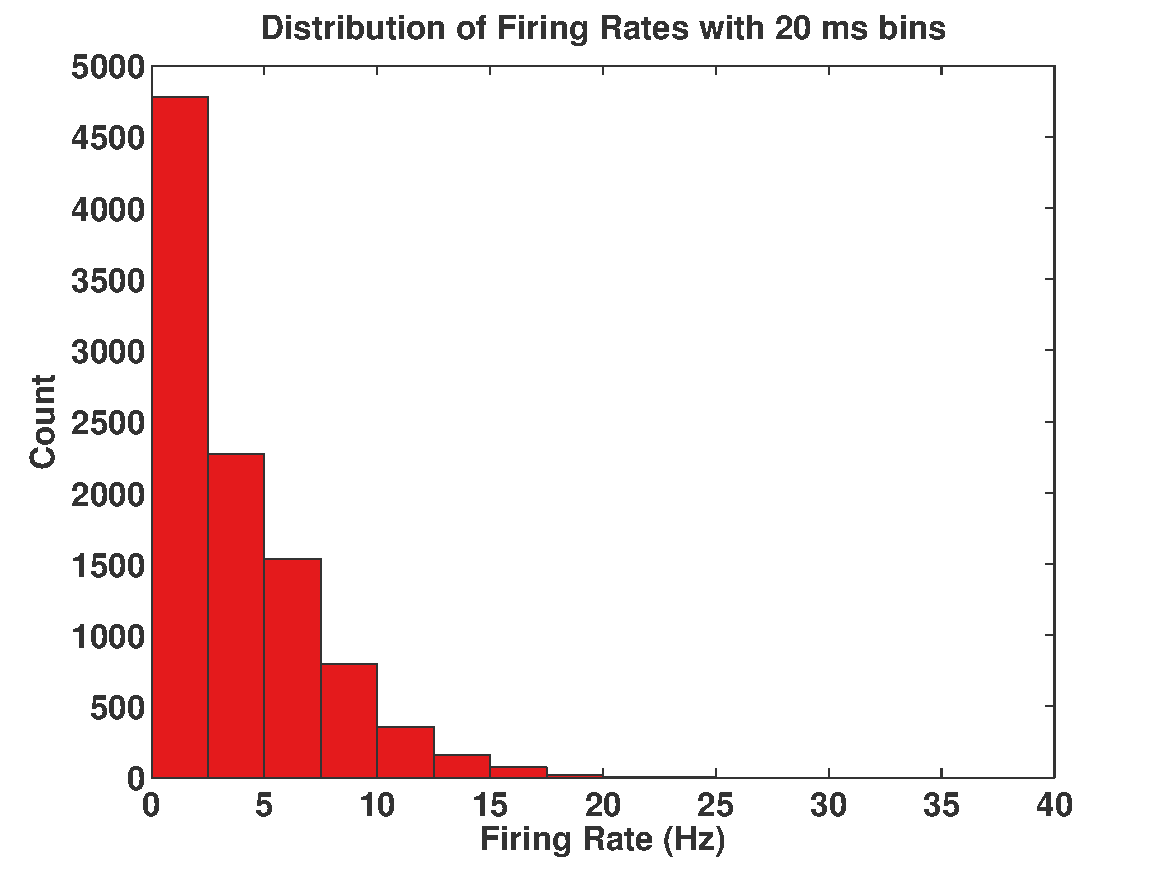
\includegraphics[width=\textwidth]{NonGaussianFR.pdf}
\end{minipage}
\begin{minipage}[b]{0.45\linewidth}
\centering
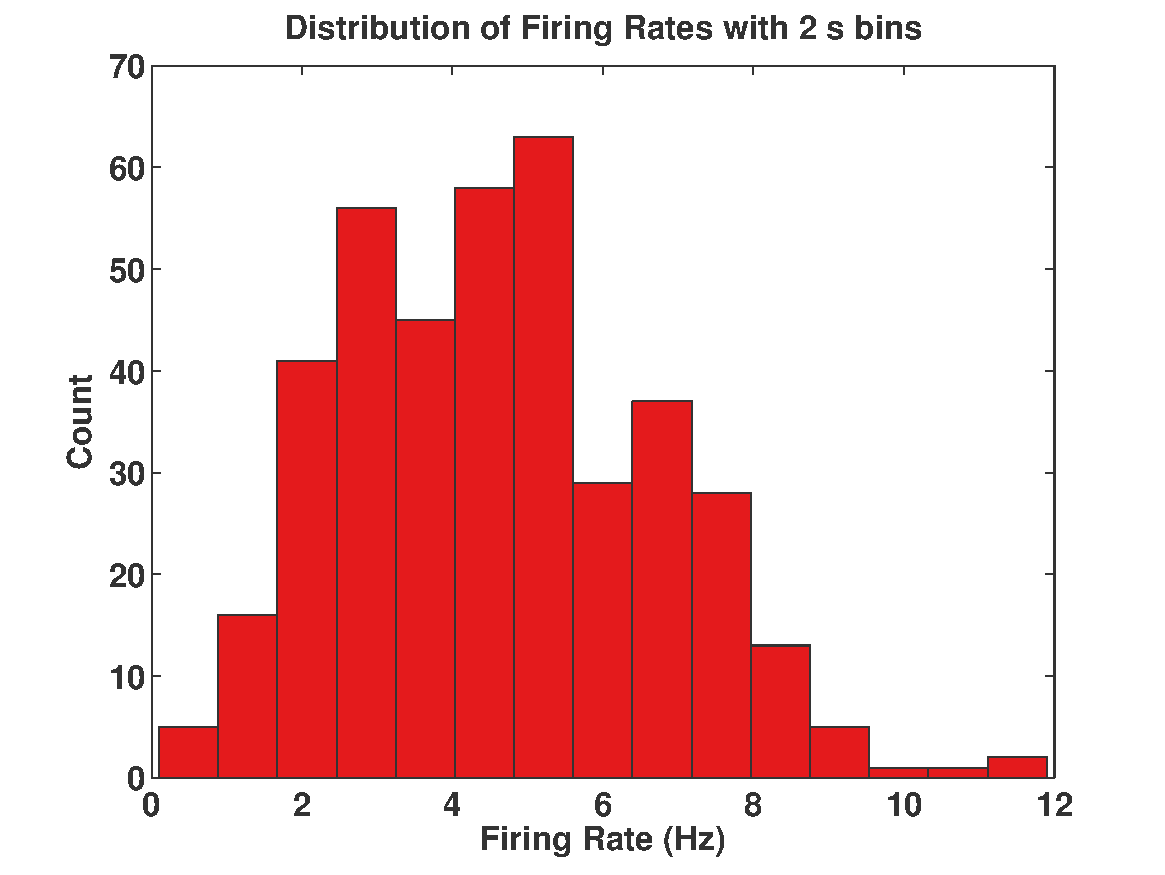
\includegraphics[width=\textwidth]{NonGaussianFR_2s.eps}
\end{minipage}
\caption{Firing rates are strongly non-Gaussian for bin sizes $<$ 1 second (left), with non-zero kurtosis persisting in distributions for larger bins (right).}
\label{Figure 5}
\end{figure}

To replicate their findings under less restrictive assumptions on the firing rate, we implemented a full spatiotemporal LNP model (Figure 6) and varied the threshold and gain under various conditions.

\begin{figure}[h!!]
\centering
\begin{minipage}[b]{0.48\linewidth}
\centering
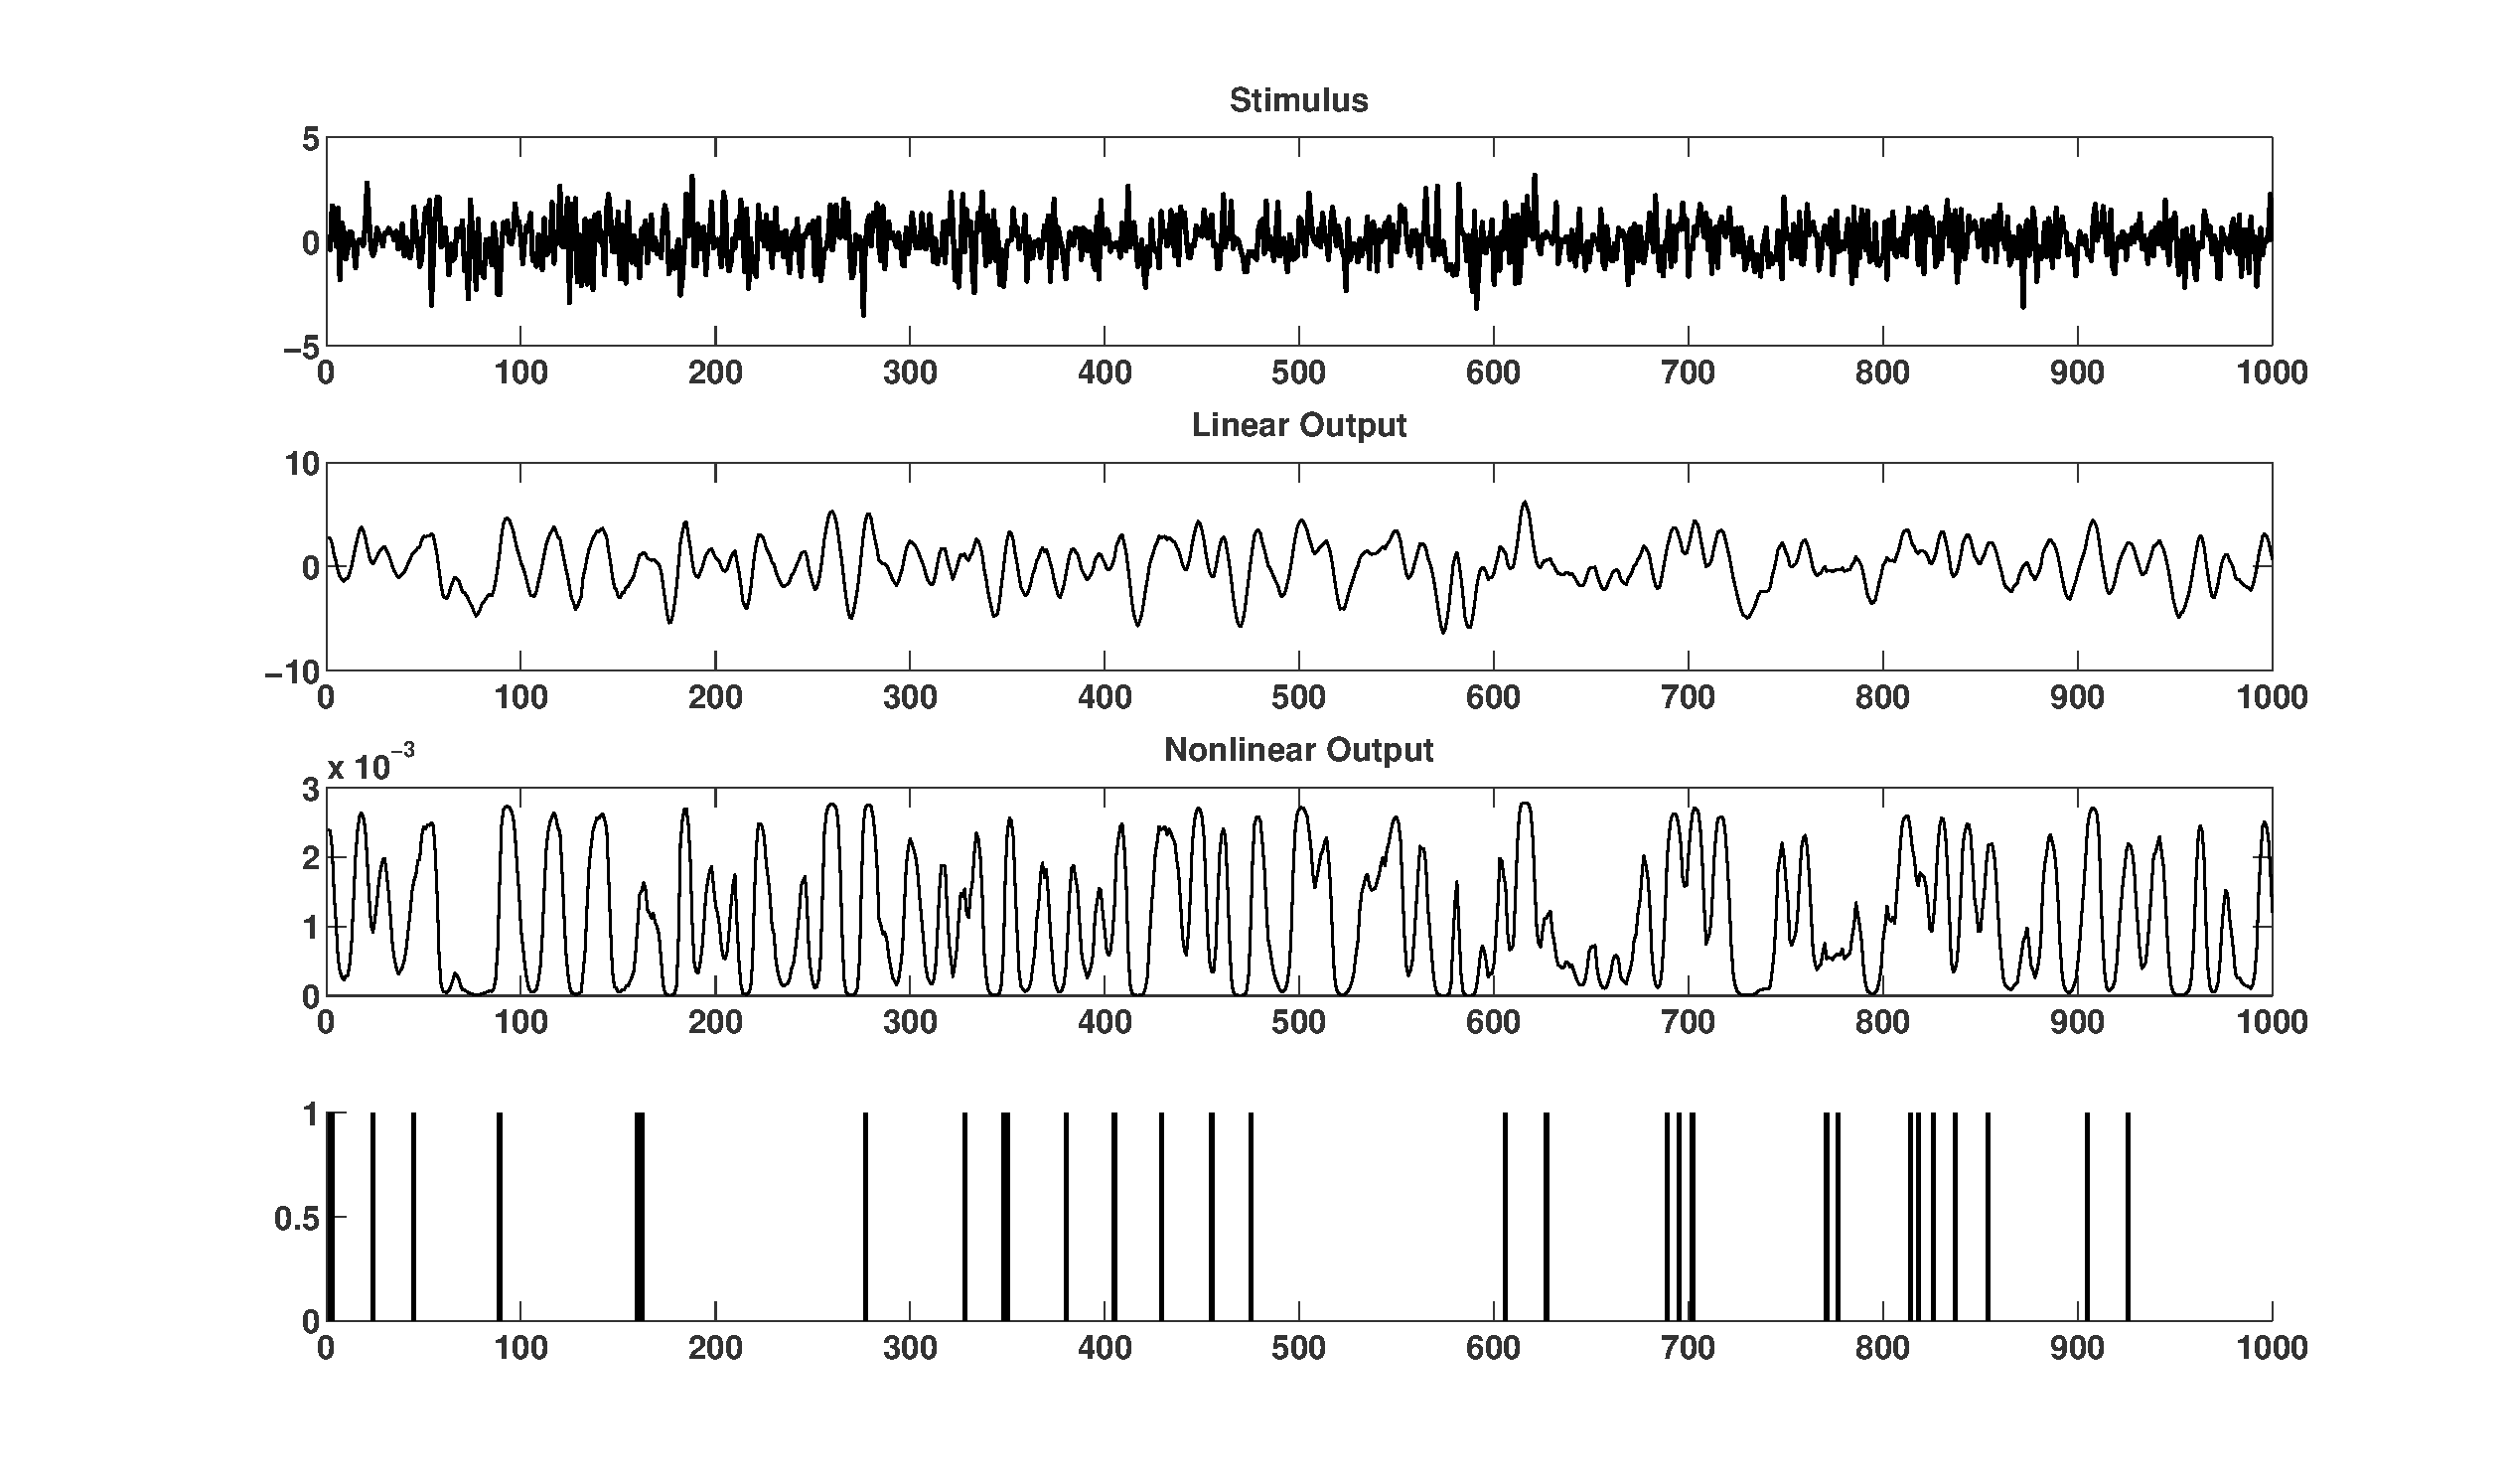
\includegraphics[width=\textwidth]{lnp_white.eps}
\end{minipage}
\begin{minipage}[b]{0.48\linewidth}
\centering
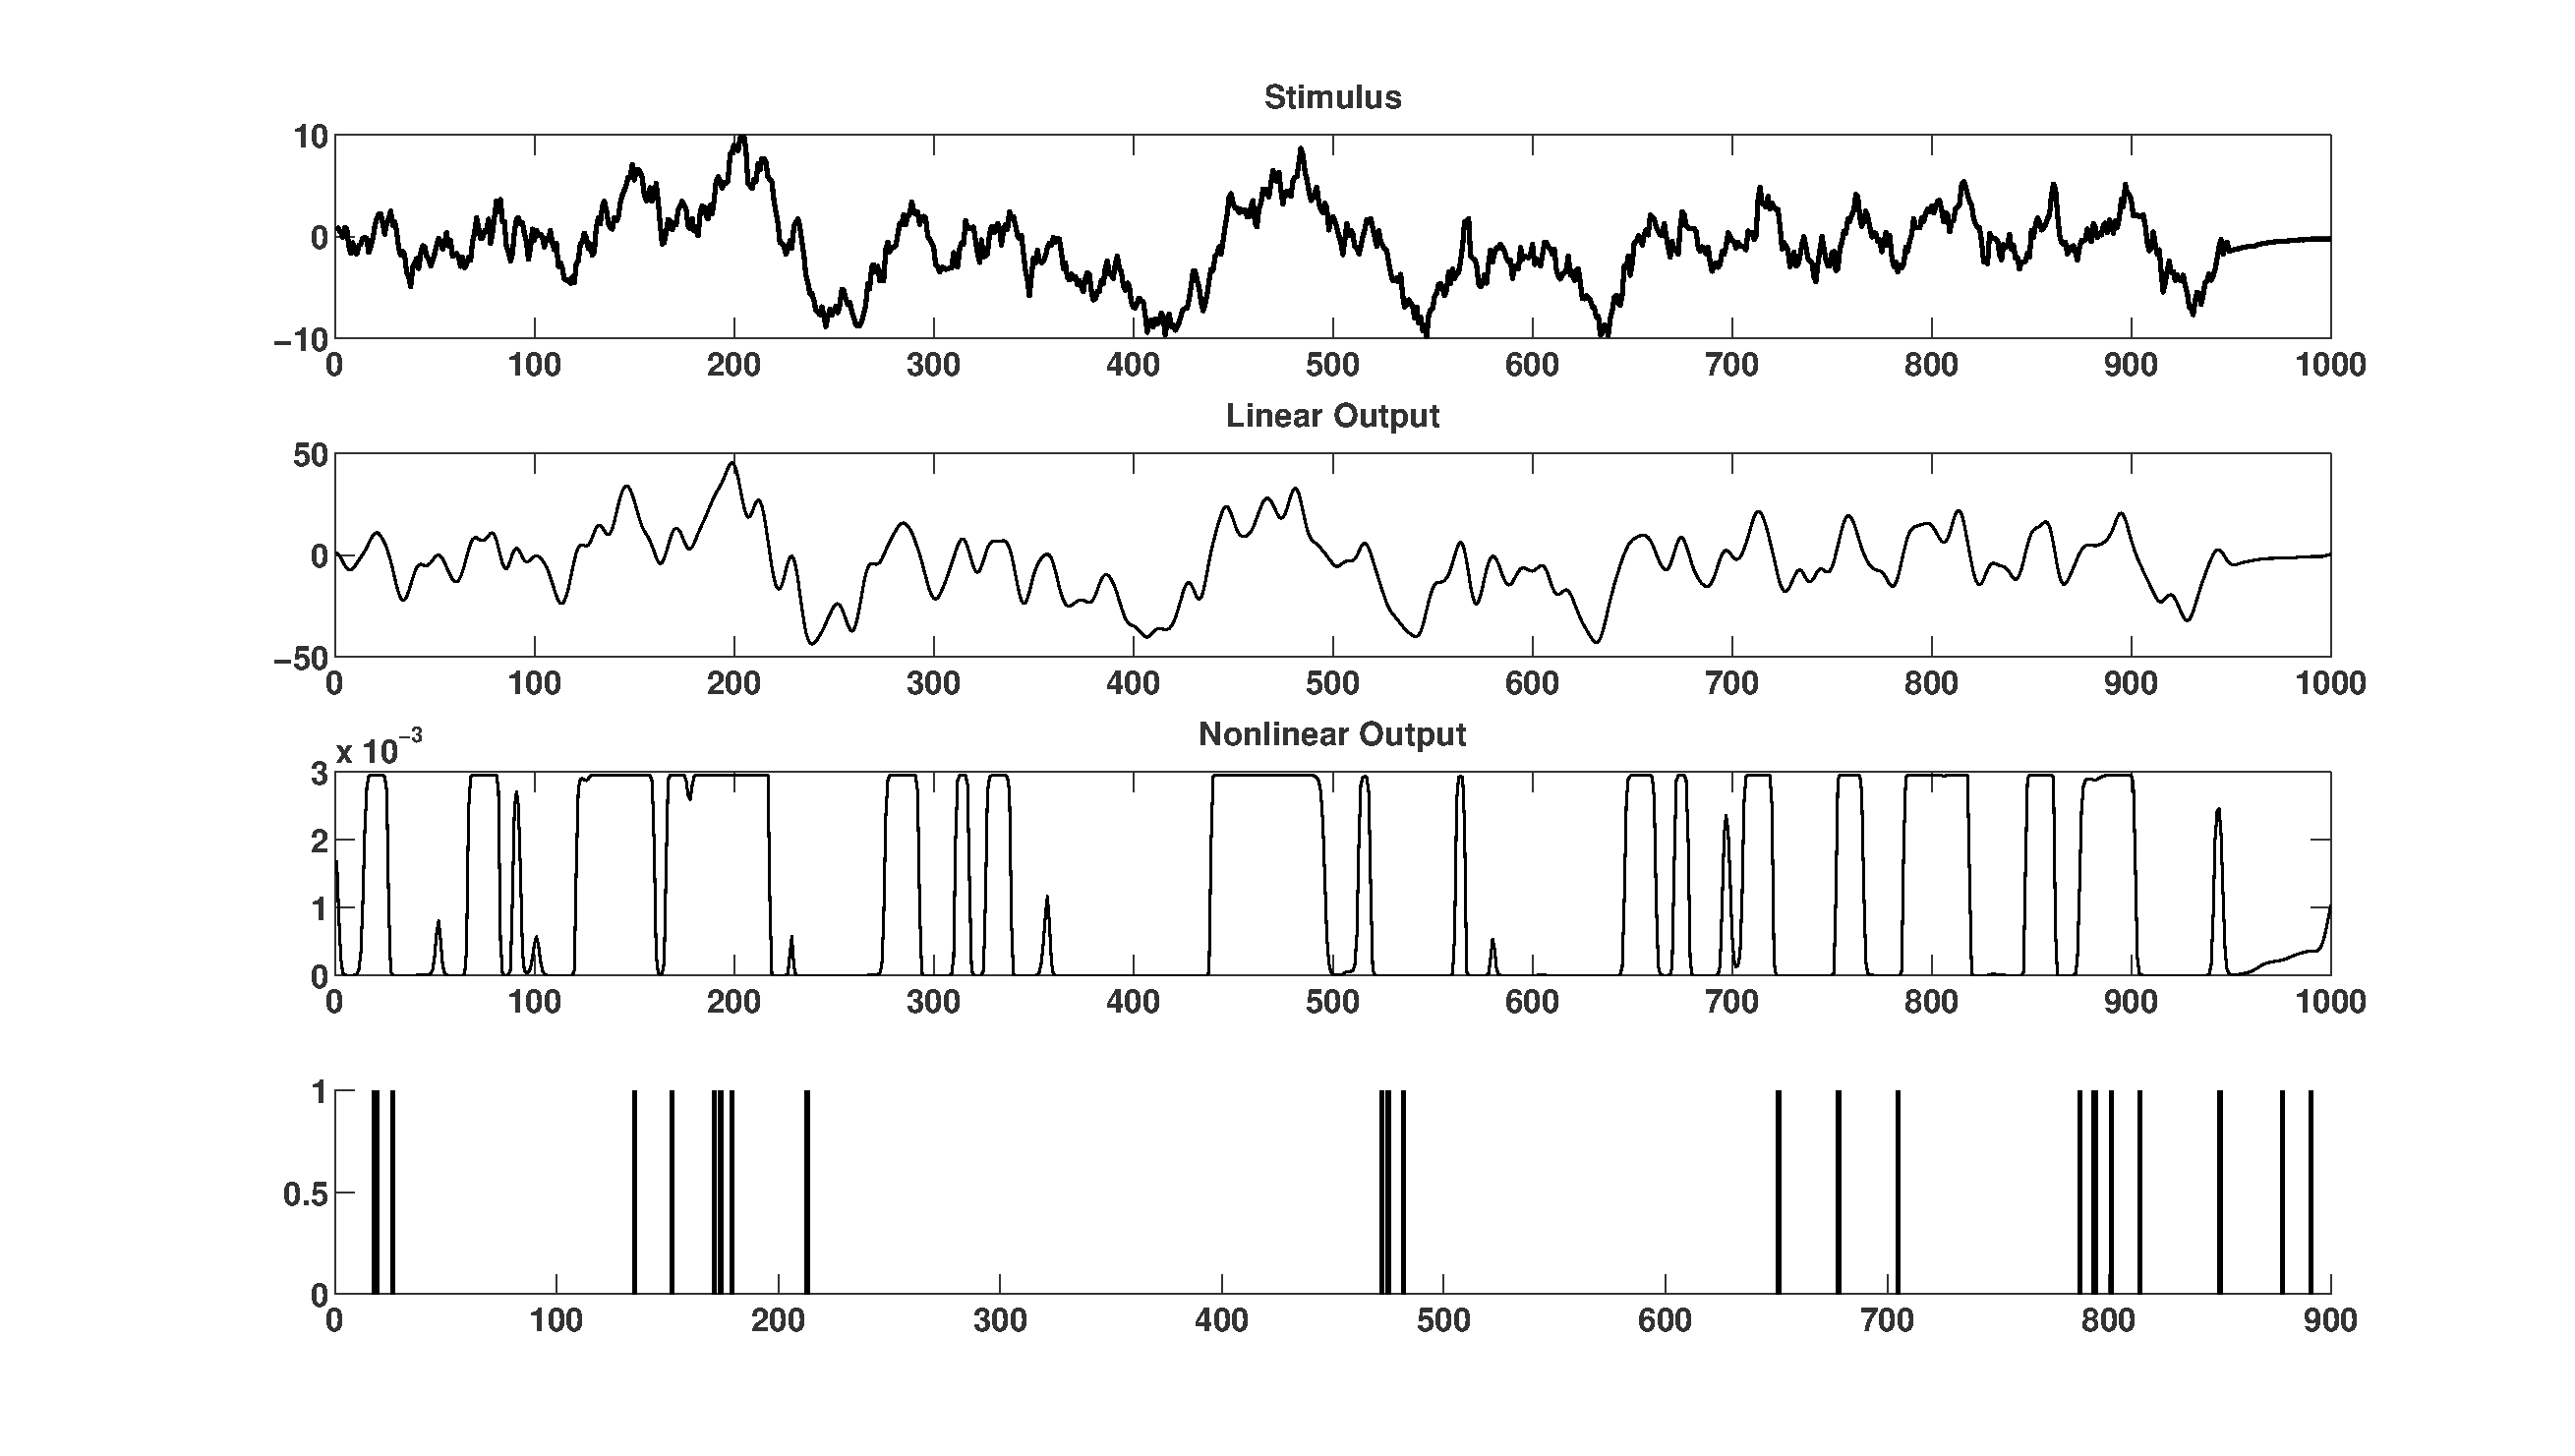
\includegraphics[width=\textwidth]{lnp_pink.eps}
\end{minipage}
\caption{The various stages of an LNP model responding to white noise (left) and white noise convolved with a decaying exponential filter to lend it temporal correlations (right).  In both plots the first line is the stimulus, the second is the linear output after the stimulus is convolved with the (monophasic or biphasic) linear filter, and the third is the nonlinear output of the sigmoid function taking the linear output as its argument.  The fourth and last line is the spiking output generated by Matlab's poisson random number generator with $\lambda$ proportional to the nonlinear output.}
\label{Figure 5}
\end{figure}



\section{Methods}

\subsection{Idealized LNP Model}

Note: In this section, numbered equations are taken from the Pitkow Meister paper. This is a description of the equations from that paper and how they enabled us to examine the effect of various parameters on mutual information and correlation.

\subsubsection{Mutual Information}

The reduced LNP model works under the assumption that the firing rate is a deterministic function of the stimulus, i.e. that the input noise is negligible. With this assumption, the mutual information between the spike count, $n$, and the stimulus, $s$, is equivalent to the mutual information between the spike count and the firing rate, $\rho$.

\begin{align}
\displaystyle I(n;s) = H(n)-H(n|s)=H(n)-H(n|\rho)=I(n;\rho) \tag{18}
\end{align}

\noindent Now that we have this equivalency, we only need to calculate the probability distributions for the firing rate and the spike count, and calculate the mutual information between them. We start with the linear output of the LNP model, $r$, which we assume to be normally distributed with mean 0 and variance 1. This will be true by construction due to the statistics of the stimulus. Therefore, $r$ has the standard Gaussian probability distribution

\begin{align}
\displaystyle p(r) = \frac{1}{\sqrt{2\pi}}e^{-r^2/2} \notag
\end{align}

\noindent This output is passed through a sigmoidal nonlinearity with peak $K$, gain $g$, and half-max threshold $\theta$ to get the firing rate, $\rho$.

\begin{align}
\displaystyle \rho(t) = N(r(t)) = K \Big/ \left(1+e^{-g(r(t)-\theta)}\right) \tag{8, 10}
\end{align}

\noindent We can derive the probability distribution for $\rho$ by changing variables from $r$ to $\rho$. Note that $r=N^{-1}(\rho)$.

\begin{align}
\displaystyle p(\rho) = p(N^{-1}(\rho))\left | \frac{dN^{-1}(\rho)}{d\rho} \right | \notag
\end{align}

\noindent Since $\displaystyle N^{-1}(\rho)= \theta - \log(K/\rho-1)$ by equation 10, this yields the following formula for the distribution of firing rates:

\begin{align}
\displaystyle p(\rho) = \frac{K\exp\left[ -\frac{1}{2}\left( \frac{1}{g}\log(K/\rho-1)-\theta\right)^2\right]}{\sqrt{2\pi}g\rho^2(K/\rho-1)} \tag{19}
\end{align}

\noindent The distribution of spike counts is assumed to be Poisson, with mean equal to the firing rate times the length of the time window.
\begin{align}
\displaystyle P(n|\rho) = \frac{e^{-\rho\Delta t}(\rho \Delta t)^n}{n!} \tag{9}
\end{align}

\noindent To find the unconditional probability of observing $n$ spikes in a time window, we integrate over all possible values of $\rho$.

\begin{align}
\displaystyle P(n) =\int d\rho \; P(n|\rho) \; p(\rho) \notag
\end{align}

\noindent Now we can calculate mutual information between the spike count and the firing rate using $I(n;\rho)=H(n)-H(n|\rho)$, where $H(n)$ and $H(n|\rho)$ are given by

\begin{align}
\displaystyle H(n) = -\sum\limits_{n=0}^\infty P(n)\log P(n) \tag{16}
\end{align}

\begin{align}
\displaystyle H(n|\rho) = -\int\limits_0^K d\rho \; p(\rho) \sum\limits_{n=0}^\infty P(n|\rho) \log P(n|\rho) \tag{17}
\end{align}

\noindent The integral goes from zero to $K$ in equation 17 because $K$ is the peak firing rate. This enables us to calculate mutual information as a function of gain ($g$), threshold ($\theta$), and peak rate ($K$), which enter into the formula for $I(n;\rho)$ via equation 19. Bits per spike is simply $I(n;\rho)/n$.

\subsubsection{Correlation}

Suppose that two neurons have linear outputs $x$ and $y$ that are normally distributed with mean zero, variance one, and correlation coefficient $c$. Then the covariance matrix is

\[ {\bf\Sigma} = \left( \begin{array}{cc}
1 & c \\
c & 1 \\
\end{array} \right) \]

\noindent and the joint probability distribution is

\begin{align}
\displaystyle P(x,y) = \frac{1}{2\pi |{\bf \Sigma}|^{\frac{1}{2}}}\exp\left( -\frac{1}{2}{\bf x}^T {\bf \Sigma}^{-1} {\bf x}\right)=\frac{1}{2\pi \sqrt{1-c^2}}\exp\left( -\frac{1}{2}\frac{x^2-2xyc+y^2}{1-c^2}\right) \tag{13}
\end{align}

\noindent When we pass this through the nonlinearity $N$ (equation 10), the correlation becomes

\begin{align}
\displaystyle C_{N(x)N(y)} = \frac{\langle N(x)N(y)\rangle- \langle N(x)\rangle^2}{\langle N(x)^2 \rangle - \langle N(x) \rangle^2} \tag{12}
\end{align}

\noindent where $\langle \:\rangle$ denotes expected value. This equation makes use of the fact that $\langle N(x) \rangle = \langle N(y) \rangle$ and $\langle N(x)^2 \rangle = \langle N(y)^2 \rangle$. These expected values are calculated by numerical integration:

\begin{align}
\langle N(x)N(y) \rangle = \int \int dx\;dy\;N(x)N(y)P(x,y) \notag
\end{align}

\noindent This enables us to calculate the amount by which the nonlinearity reduces correlations that are present at the output of the linear filter.

\subsection{Full LNP Model}



\newpage
\begin{thebibliography}{9}


\bibitem{Dan} Dan, Y., Atick, J., and Clay R. (1996) Efficient coding of natural scenes in the lateral geniculate nucleus: experimental test of a computational theory. \textit{The Journal of Neuroscience} 16(10): 3351-3362.

\bibitem{Puchalla} Puchalla, J., Schneidman, E., Harris, R., and Berry, M. (2005) Redundancy in the population code of the retina. \textit{Neuron} 46: 493-504

\bibitem{Pitkow} Pitkow, X., and Meister, M. (2012) Decorrelation and efficient coding by retinal ganglion cells. \textit{Nature Neuroscience} 15(4): 628-635.


\end{thebibliography}


\end{document}